\documentclass[xetex]{beamer}

\mode<presentation> {
  \usetheme{Frankfurt}
  \setbeamercovered{transparent}
}

\usepackage{xunicode}
\usepackage{xltxtra}
\usepackage[czech]{babel}
\usepackage{palatino}
\usepackage{graphicx}
\usepackage{textpos}

\usepackage{listings}
\lstset{language=bash,
        numbers=left,
        numberstyle=\tiny,
        showstringspaces=false,
        aboveskip=-40pt,
        frame=leftline
        }

\title{Bitcoin}

\author{Karel Bílek\\Ondřej Profant}
\institute[Piráti]{Česká pirátská strana}
\date{\today}

\begin{document}

\begin{frame}
	\begin{textblock*}{0cm}(-1cm,-3.78cm)
  
\includegraphics[scale=0.6]{images/intro.jpg}
  \end{textblock*}
\end{frame}

\begin{frame}
  \titlepage
\end{frame}

\begin{frame}
  \frametitle{Osnova}
  \tableofcontents
\end{frame}	

\begin{frame}
	\frametitle{Disclaimer}
	Bitcoin je poměrně složité téma, proto není lehké připravit prezentaci, která by nepůsobila poněkud chaoticky
	a~přesto nemusela zjednodušovat.

	\bigskip

	Předem se proto omlouváme za podobné nedostatky přednášky.

	\bigskip

	Pokud máte konstruktivní připomínky či dokonce konkrétní nápady, jak prezentaci vylepšit, tak kontaktujte autory, či rovnou pošlete pull request na Githubu.
\end{frame}

\section{Základní charakteristika}

\begin{frame}
	\frametitle{Základní charakteristika}

	Co je Bitcoin?
	\begin{itemize}
		\item<1-4> měna
		\item<2-4> \textbf{crypto}měna
		\item<3-4> \textbf{decentralizovaná} cryptoměna
		\item<4-4> decentralizovaná \textbf{cyber}cryptoměna
	\end{itemize}
\end{frame}

\begin{frame}
 	\frametitle{Základní charakteristika}
	\begin{itemize}
		\item bezpečná: podložena výpočetním výkonem (šiframa)
		\item globální: velmi nízké poplatky za libovolnou transakci
		\item volnost: každý může mít zdarma neomezený počet peněženek
		\item anonymita: resp. pseudoanonymita
		\item transparentí: všechny transakce jsou veřejné
		\item předem dané množství Bitcoinů $\Rightarrow$ deflační měna (?)
	\end{itemize}
\end{frame}

\section{Praktické použití}

\begin{frame}
	\frametitle{Praktické použití}
	Adresa je hash, např: 19bRk3XRrAfeE1Z1zr1C9M8n7d1PygHDYZ

	\bigskip

	Před provedením transakce určíme poplatek (fee). Lze i 0. Výše poplatku ovlivní rychlost potvrzení transakce.
\end{frame}

\begin{frame}
 \frametitle{Praktické použití}
	klienti
\end{frame}

\section{Čím je měna podložena}

\begin{frame}
	\frametitle{Čím je měna podložena}

	Blockchain je vícenásobně zahashovaná historie všech transakcí. 

	\bigskip

	Když provedeme transakci, tak se přidá do blockchainu. 

	\bigskip

	Mineři pátrají po hashy, který ho splňuje.
\end{frame}

\begin{frame}
	\frametitle{Odbočka: hash}
	
	\begin{block}{Definice}
	Hašovací funkce je matematická funkce (resp. algoritmus) pro převod vstupních dat do (relativně) malého čísla. Výstup hašovací funkce se označuje výtah, miniatura, otisk, fingerprint či hash (česky též někdy jako haš).
	\end{block}

	\bigskip

	Stručně laicky: Hash převede libovolná data (text) na text pevně dané délky. 

	\bigskip

	Převod text $\rightarrow$ hash je rychlý. Opačně je náročný (je třeba zkoušet kombinace).

\end{frame}

\begin{frame}
	\frametitle{Čím je měna podložena}
	Miner (těžař) je osoba, která řeší umělý problém zpětného odhalení hashe.

	\bigskip

	Celkově se tím do sítě Bitcoinů dostává ohromný výpočetní výkon. Který snad garantuje dostatečnou jedinečnost.

	\bigskip

	Pokud by někdo vlastnit nadpolovičný výkon, tak by se mu mohlo podařit potvrzovat neoprávněné transakce (avšak nikoliv zrušit staré).

	\bigskip

	Za svou snahu dostávají mineři dvě odměny (vždy za vypočítaný blok):
	\begin{itemize}
		\item fee (poplatek) z transakcí
		\item nově uvolněné peníze (odměnu)
	\end{itemize}
\end{frame}

\begin{frame}
	\frametitle{Odbočka: způsob emitování pěnez}
	Bitcoinů je předem daný přesný počet.

	\bigskip
	
	Uvolňovány jsou postupně.

	\bigskip

	Tato odměna je uměle snižována. Postupem času bude miniaturní a~síť bude konvergovat k~max. počtu uvolněných bitcoinů.
\end{frame}

\begin{frame}
	\frametitle{Čím je měna podložena}
	Těžba je dnes již extrémně náročná. 

	\bigskip

	Rozhodně se nevyplatí na procesoru. Je potřeba výkoná grafická karta (navíc AMD).

	\bigskip 

	I přesto se mineři raději spojují do poolů.
\end{frame}

\begin{frame}
	\frametitle{Čím je měna podložena}
	
	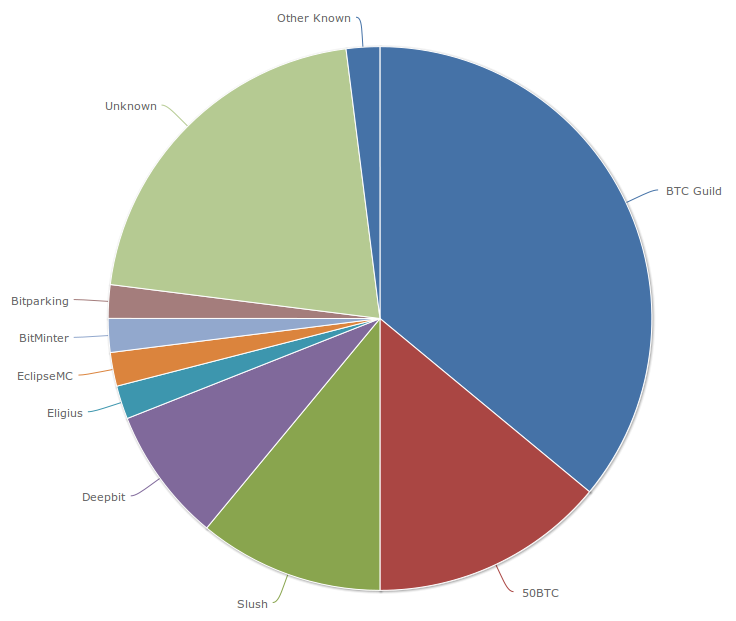
\includegraphics[scale=0.25]{images/bitcoin-pools.png}

	Přelom března/dubna 2013.

	Zdroj: \url{http://blockchain.info/pools}
\end{frame}

\begin{frame}
	\frametitle{Co lze za Bitcoin koupit}
	\begin{itemize}
		\item VPS
		\item připojení k internetu
		\item HW
		\item sázet v kasinu
		\item drogy
	\end{itemize}
\end{frame}

\begin{frame}
	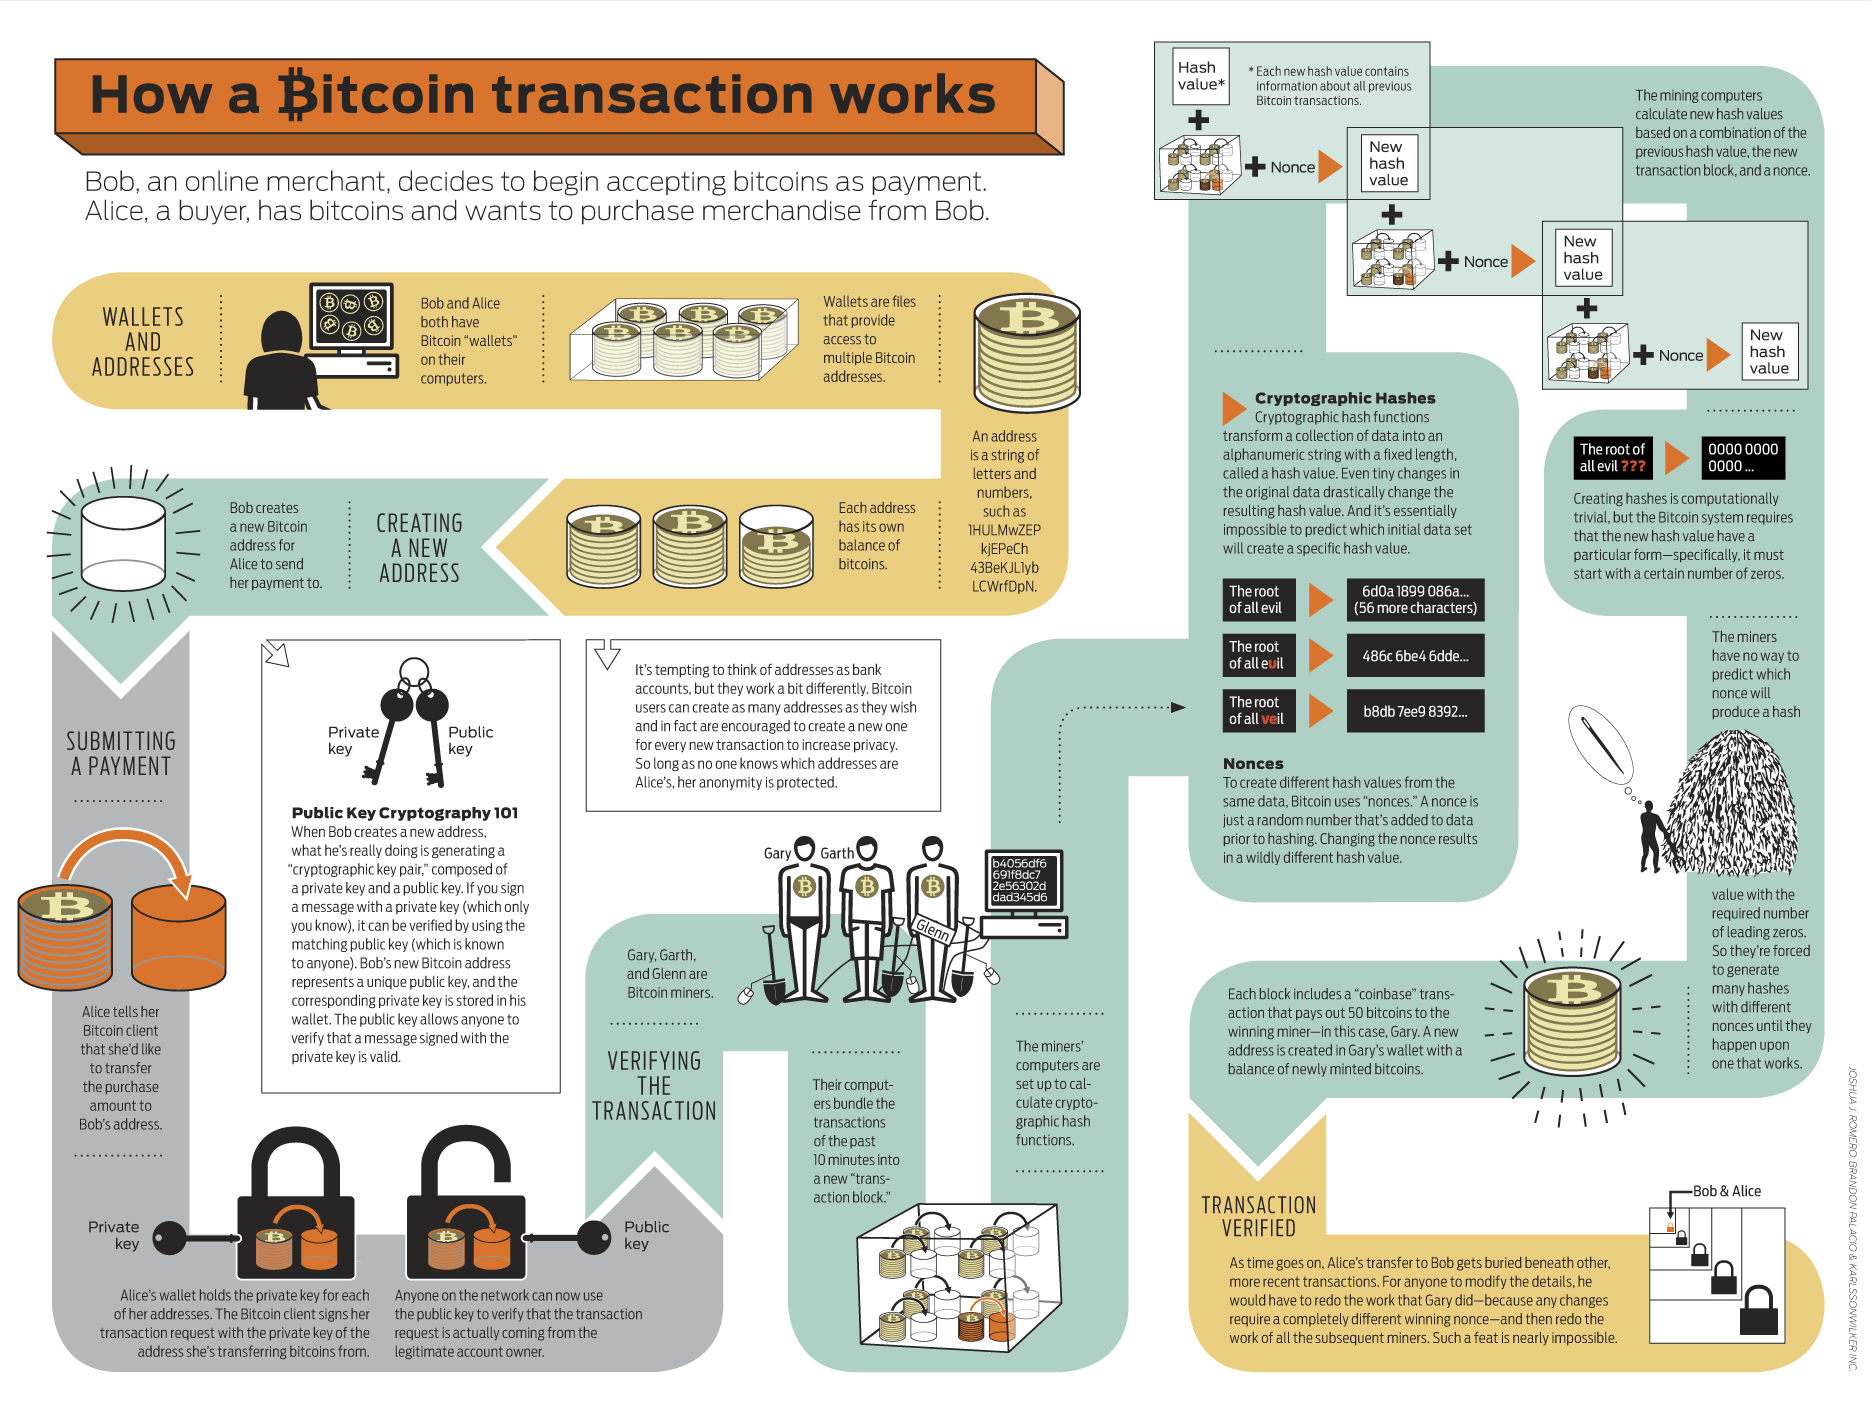
\includegraphics[scale=0.37]{images/how-a-bitcoin-transaction-works.jpg}
\end{frame}

\section{Historie}

\begin{frame}
  \frametitle{Historie}
	\begin{itemize}
		\item srpen 2008: registrována doména bitcoin.org 
		\item říjen 2008: Bitcoin design paper published 
		\item listopad 2008: Bitcoin project registered at SourceForge.net 
		\item leden 2009: First Bitcoin transaction, in block 170 - from Satoshi to Hal Finney
		\item květen 2010: laszlo first to buy pizza with Bitcoins agreeing upon paying 10,000 BTC for ~\$25 worth of pizza courtesy of jercos
	\end{itemize}

	Více na: \url{https://en.bitcoin.it/wiki/History}
\end{frame}

\begin{frame}
	\frametitle{Kurz}
	Vývoj kurzu červen 2011 až květen 2014:
	
	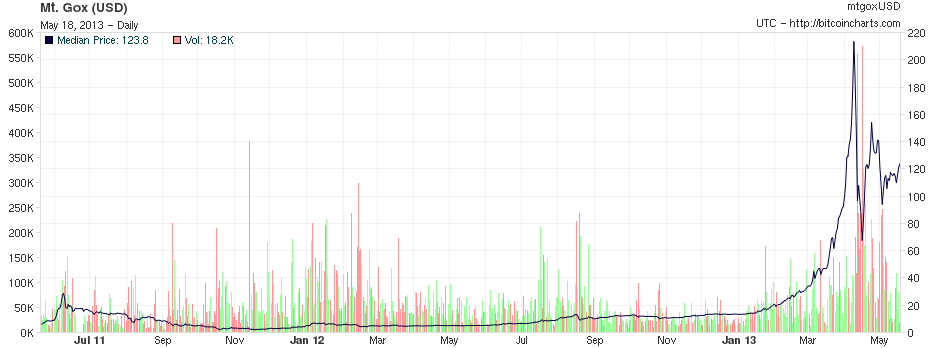
\includegraphics[scale=0.35]{images/bitcoin-exchange-rate.png}
	
\end{frame}

\begin{frame}

	Děkuji za pozornost.

	\bigskip
	
	Doplňující otázky?

	\bigskip

	\bigskip

	\scriptsize
	Copyleft Karel Bílek, Ondřej Profant, 2013. Všechna práva vyhlazena. Sdílejte, upravujte a~nechte sdílet za stejných podmínek. 

	\bigskip

	Prezentace v~úplné formě\footnote{i se zdrojovými kódy} na:\\ 
	\url{https://www.github.com/kedrigern/prezentace-cs}.

	\bigskip

	Mail: ondrej.profant -at- pirati.cz 
\end{frame}

\end{document}
